\addcontentsline{toc}{chapter}{Занятие 5. Винеровский процесс}
\chapter*{Занятие 5. Винеровский процесс}

\addcontentsline{toc}{section}{Контрольные вопросы и задания}
\section*{Контрольные вопросы и задания}

\subsubsection*{Приведите определение винеровского процесса.}

$ \left\{ w \left( t \right), \, t \geq 0 \right\} $ --- винеровский процесс,
если обладает рядом свойств:
\begin{enumerate}
  \item $w \left( 0 \right) = 0$;
  \item однородные приращения.
  Рассмотрим приращение винеровского процесса на $t$.
  Тогда
  $w \left( s + t \right) - w \left( s \right) \overset{def}{=}
    w \left( t \right) \sim
    N \left( 0, t \right) $, то есть распределение процесса зависит только от длины отрезка;
  \item независимые приращения на непересекающихся отрезках.
  Выберем $0 < t_1 < t_2 < \dotsc < t_n$.
  Тогда
  $w \left( t_1 \right), \,
    w \left( t_2 \right) - w \left( t_1 \right),
    \dotsc,
    w \left( t_n \right) - w \left( t_{n - 1} \right) $ ---
  независимые в совокупности случайные величины.
\end{enumerate}

\subsubsection*{Запишите плотность винеровского процесса.}

Напишем плотность распределения вектора
$ \left( w \left( t_1 \right), \dotsc, w \left( t_n \right) \right) =
  \vec{ \xi }$.

Будем использовать матрицу
$$A =
  \begin{bmatrix}
    1 & 0 & 0 & 0 & \dotsc & 0 \\
    1 & 1 & 0 & 0 & \dotsc & 0 \\
    1 & 1 & 1 & 0 & \dotsc & 0 \\
    \dotsc \\
    1 & 1 & 1 & 1 & \dotsc & 1
  \end{bmatrix}.$$

Таким образом $ \vec{ \xi }$ имеет плотность
$$q \left( A^{-1} \vec{u} \right) =
  \prod \limits_{j = 0}^{n - 1}
    \frac{1}{ \sqrt{2 \pi \left( t_{j + 1} - t_j \right) }} \cdot e^{-\frac{u_{j + 1} - u_j}{2t_{j + 1} - t_j}}.$$
В этой плотности считаем, что $t_0 = 0, \, u_0 = 0$.

\subsubsection*{Запишите ковариационную функцию винеровского процесса.}

Произведение математических ожиданий --- это 0, потому
$$K \left( t, s \right) =
  Mw \left( s \right) w \left( t \right) =$$
Используем независимость приращений
$$= M \left\{
    w \left( s \right) \cdot
    \left[ w \left( s \right) + \left( w \left( t \right) - w \left( s \right) \right) \right]
  \right\} =$$
Раскрываем скобки
$$= M \left\{
    w^2 \left(s \right) + Mw \left( s \right) \left[ w \left( t \right) - w \left( s \right) \right]
  \right\} =$$
Первое слагаемое равно $s$, а второе --- нулю,
так как это независимые центрированные случайные величины (математическое произведения ---
это произведение математических ожиданий, а они равны нулю)
$$= s, \,
  s < t.$$

$K \left( t, s \right) = \min \left( s, t \right) $.

\addcontentsline{toc}{section}{Аудиторные задачи}
\section*{Аудиторные задачи}

\subsubsection*{5.2}

\textit{Задание.}
Пусть $ \left\{ W \left( t \right), \, t \geq 0 \right\} $ --- винеровский процесс.
Докажите, что
$M \left( W \left( t \right) - W \left( s \right) \right)^{2n + 1} = 0, \,
  M \left( W \left( t \right) - W \left( s \right) \right)^{2n} =
  \left( 2n - 1 \right)!! \left( t - s \right)^n$.

\textit{Решение.}
Приращение гауссовское.
Обозначим
$$ \xi =
  W \left( t \right) - W \left( s \right) \overset{def}{=}
  W \left( t - s \right).$$
Значит, $ \xi \sim N \left( 0, t - s \right) $, где $t - s = \sigma^2$.
Нужны формулы для моментов центрированной гауссовской случайной величины, то есть
Знаем, что $M \xi^{2n + 1} = 0, \, M \xi^{2n} = \left( 2n + 1 \right)!! \sigma^{2n}$.

\subsubsection*{5.3}

\textit{Задание.}
Пусть $ \left\{ W \left( t \right), \, t \geq 0 \right\} $ --- винеровский процесс.
Вычислите:
\begin{enumerate}[label=\alph*)]
  \item $M \left[ \left( W \left( 5 \right) - 2W \left( 1 \right) + 2 \right)^3 \right] $;
  \item характеристическую функцию случайной величины $W \left( 2 \right) + 2W \left( 1 \right) $;
  \item $M \left[ \sin \left( 2W \left( 1 \right) + W \left( 2 \right) \right) \right] $;
  \item $M \left[ \cos \left( 2W \left( 1 \right) + W \left( 2 \right) \right) \right] $.
\end{enumerate}

\textit{Решение.}
Есть винеровский процесс.
\begin{enumerate}[label=\alph*)]
  \item $W \left( 5 \right) - 2W \left( 1 \right) + 2 = \xi \sim N \left( 2, 5 \right) $,
  потому что это линейная комбинация элементов гауссовского вектора.
  Найдём дисперсию.
  Константа на неё не влияет
  $$D \xi =
    D \left[ W \left( 5 \right) - 2W \left( 1 \right) \right] =
    cov \left( \xi, \xi \right) =$$
  Подставим выражения для случайной величины
  $$= cov \left[ W \left( 5 \right) - 2W \left( 1 \right) + 2, \,
      W \left( 5 \right) - 2W \left( 1 \right) + 2 \right] =$$
  Воспользуемся линейностью
  $$= K \left( 5, 5 \right) - 2K \left( 5, 1 \right) - 2K \left( 5, 1 \right) +
    4K \left( 1, 1 \right) =
    5 - 2 - 2 + 4 =
    5.$$
  Нужно найти третий момент.
  $ \xi $ не центрирована.
  Нужно её центрировать $M \xi^3 = M \left[ \left( \xi - 2 \right) + 2 \right]^3 $.
  Раскрываем скобки
  $$M \xi^3 =
    M \left( \xi - 2 \right)^3 + 6M \left( \xi - 2 \right)^3 + 12M \left( \xi - 2 \right) + 8.$$
  По предыдущей задаче первое слагаемое --- 0, так как величина центрирована, второй момент --- 5,
  так как это дисперсия, первый момент --- 0.
  Тогда $M \xi^3 = 0 + 6 \cdot 5 + 12 \cdot 0 + 8 = 38$.

  Величины $W \left( 5 \right) $ и $W \left( 1 \right) $ --- зависимы,
  а приращения в винеровском процессе --- независимы, потому имеем сумму дисперсий
  $$D \left[ W \left( 5 \right) - 2W \left( 1 \right) \right] =
    D \left\{
      \left[ W \left( 5 \right) - W \left( 1 \right) \right] + \left[ -W \left( 1 \right) \right]
    \right\}.$$
  Дисперсия первого слагаемого равна 4, а второго --- 1.
  Слагаемые независимы $D \left[ W \left( 5 \right) - 2W \left( 1 \right) \right] = 5$;
  \item нужно найти характеристическую функцию $W \left( 2 \right) + 2W \left( 1 \right) $.

  Математическое ожидание такой величины равно нулю, а дисперсия
  $D \left[ W \left( 2 \right) + 2W \left( 1 \right) \right] =
    D \left\{
      \left[ W \left( 2 \right) - W \left( 1 \right) \right] + 3W \left( 1 \right)
    \right\}$.
  Это независимые величины, поэтому
  $D \left\{
      \left[ W \left( 2 \right) - W \left( 1 \right) \right] + 3W \left( 1 \right)
    \right\} =
    1 + 9 = 10$.
  Значит, получается
  $ \varphi_{W \left( 2 \right) + 2W \left( 1 \right) } \left( \lambda \right) =
    \varphi_{N \left( 0, 10 \right) } \left( \lambda \right) =
    e^{-\frac{10 \lambda^2}{2}}$;
  \item $M \left[ \sin \left( 2W \left( 1 \right) + W \left( 2 \right) \right) \right] = 0$.

  Характеристическая функция случайной величины --- это
  $$ \varphi_{ \xi } \left( \lambda \right) = Me^{i \lambda \xi } =
    M \cos \lambda \xi + iM \sin \lambda \xi, \,
    \lambda = 1;$$
  \item $M \left[ \cos \left( 2W \left( 1 \right) + W \left( 2 \right) \right) \right] = e^{-5}$.
\end{enumerate}

\subsubsection*{5.4}

\textit{Задание.}
Пусть $ \left\{ W \left( t \right), \, t \geq 0 \right\} $ --- винеровский процесс.
Докажите, что процессы
\begin{enumerate}[label=\alph*)]
  \item $ \left\{ -W \left( t \right), \, t \geq 0 \right\} $;
  \item $ \left\{ W \left( s + t \right) - W \left( s \right), \, t \geq 0 \right\} $;
  \item $ \tilde{W} \left( t \right) =
    tW \left( \frac{1}{t} \right) \cdot \mathbbm{1} \left\{ t > 0 \right\} $
\end{enumerate}
тоже являются винеровскими.

\textit{Решение.}
$ \left\{ W \left( t \right), \, t \geq 0 \right\} $ --- это винеровский процесс.
Нужно проверить, что некоторые преобразования винеровского процесса оставляют его винеровским.

\begin{enumerate}[label=\alph*)]
  \item Если выберем моменты времени $t_1 < \dotsc < t_n$ и возьмём вектор
  $$ \left( W \left( t_1 \right), \dotsc, W \left( t_n \right) \right) $$
  --- гауссовский.
  Нужно знать, что в каждой точке $MW \left( t \right) = 0$ и
  $$K \left( t, s \right) =
    \min \left( t, s \right).$$
  Если процесс удовлетворит этим трём свойствам, то это винеровский процесс.

  $M \left[ -W \left( t \right) \right] =
    -MW \left( t \right) =
    0$.

  Найдём ковариационную функцию
  $$K \left( t, s \right) =
    M \left[ W \left( t \right) W \left( s \right) \right] =
    \min \left( t, s \right).$$

  Вектор значений этого процесса должен быть гауссовским.
  Возьмём $ \left( -W \left( t_1 \right), \dotsc, -W \left( t_n \right) \right) $.
  Нужно сказать, что это гауссовский вектор.
  Почему?

  Этот вектор --- это линейное преобразование вектора
  $$ \left( W \left( t_1 \right), \dotsc, W \left( t_n \right) \right).$$
  Линейные преобразования оставляют вектор гауссовским;
  \item сначала нужно сказать, что у него гауссовские конечномерные распределения.

  Берём $n$ значений этого процесса
  $$ \left(
      W \left( s + t_1 \right) - W \left( s \right), \dotsc,
      W \left( s + t_n \right) - W \left( s \right)
    \right) $$
  --- гауссовский, так как этот вектор --- это линейное преобразование вектора
  $ \left( W \left( t_1 + s \right), \dotsc, W \left( t_n + s \right), W \left( s \right) \right) $.
  Что это будет за линейное преобразование?

  $$ \begin{bmatrix}
      1 & 0 & -1 \\
      0 & 1 & -1
    \end{bmatrix}
    \begin{bmatrix}
      W \left( s + t_1 \right) \\
      W \left( s + t_2 \right) \\
      W \left( s \right)
    \end{bmatrix} =
    \begin{bmatrix}
      W \left( s + t_1 \right) - W \left( s \right) \\
      W \left( s + t_2 \right) - W \left( s \right)
    \end{bmatrix}.$$

  Математическое ожидание --- 0.

  Нужно посчитать ковариационную функцию.
  Нужно проверить, что она равняется минимуму
  $$K \left( t_1, t_2 \right) =
    M \left\{
      \left[ W \left( s + t_1 \right) - W \left( s \right) \right] \cdot
      \left[ W \left( s + t_2 \right) - W \left( s \right) \right] \right\} =$$
  Перемножим скобки
  $$= M \left[
      W \left( s + t_1 \right) W \left( s + t_2 \right) -
      W \left( s + t_1 \right) W \left( s \right) - W \left( s \right) W \left( s + t_2 \right) +
      W \left( s \right)^2 \right] =$$
  Математическое ожидание первого слагаемого --- ковариация винеровского процесса.
  Она равна минимуму.
  Математическое ожидание последнего слагаемого --- ковариация в точке $ \left( s, s \right) $.
  Получаем
  $$= \min \left( s + t_1, s + t_2 \right) - s - s + s =
    \min \left( s + t_1, s + t_2 \right) - s.$$
  Можем вынести и сократить
  $\min \left( s + t_1, s + t_2 \right) - s =
    \min \left( t_1, t_2 \right) $.
  Значит, ковариация такая, как надо.
  Это винеровский процесс;
  \item берём конечномерные распределения
  $$ \left(
      t_1 W \left( \frac{1}{t_1} \right), \dotsc, t_n W \left( \frac{1}{t_n} \right)
    \right) $$
  --- гауссовский, так как это линейное преобразование вектора винеровского процесса
  $ \left( W \left( \frac{1}{t_1} \right), \dotsc, W \left( \frac{1}{t_n} \right) \right) $.

  Математическое ожидание --- 0.
  Осталось найти ковариационную функцию
  $$K \left( t, s \right) =
    M \left[ tW \left( \frac{1}{t} \right) sW \left( \frac{1}{s} \right) \right] =$$
  Выносим $t$ и $s$.
  Получаем
  $$= ts \min \left( \frac{1}{t}, \frac{1}{s} \right) =$$
  Множитель $ts$ --- положительный.
  Он вносится
  $$= \min \left( t, s \right).$$
  Получилось.
\end{enumerate}

\subsubsection*{5.5}

\textit{Задание.}
Пусть $ \left\{ W^i \left( t \right), \, t \geq 0 \right\}_{i \geq 1}$ ---
независимые винеровские процессы.
Найдите константу $c_n$ так, чтобы процесс
$$ \tilde{W} \left( t \right) =
  c_n \sum \limits_{i = 1}^n W^i \left( t \right), \,
  t \geq 0$$
был винеровским.

\textit{Решение.}
Сложили $n$ независимых винеровским процессов так, чтобы процесс был винеровским.

Скажем, что такой процесс гауссовский
\begin{gather*}
  \left( \tilde{W} \left( t_1 \right), \dotsc, \tilde{W} \left( t_n \right) \right) = \\
  = \left(
    c_n \left( W^1 \left( t_1 \right), \dotsc, W^n \left( t_n \right) \right), \dotsc,
    c_n \left( W^1 \left( t_m \right), \dotsc, W^n \left( t_m \right) \right)
  \right)
\end{gather*}
--- это линейное преобразование.

$$ \begin{bmatrix}
    W^1 \left( t_1 \right) \\
    \dotsc \\
    W^1 \left( t_m \right) \\
    W^2 \left( t_1 \right) \\
    \dotsc \\
    W^2 \left( t_m \right)
  \end{bmatrix}$$
--- гауссовский вектор, где обе части --- независимые гауссовские вектора.

Математическое ожидание такого процесса --- 0, так как математическое ожидание каждого процесса ---
0.
Посчитаем ковариацию и скажем, како должна быть $c_n.$
Ковариация линейна по каждому аргументу.
Это значит, что множители и суммы выносятся
$$cov \left(
    c_n \sum \limits_{i = 1}^n W^i \left( t \right), \,
    c_n \sum \limits_{i = 1}^n W^i \left( s \right)
  \right) =
  c_n^2 \sum \limits_{i = 1}^n
    \sum \limits_{j = 1}^n cov \left[ W^i \left( t \right), \, W^j \left( s \right) \right] =$$
Когда индексы разные --- это0, когда одинаковые --- это минимум
$$= c_n^2 \sum \limits_{i = 1}^n \min \left( t, s \right) =$$
Имеем $n$ одинаковых слагаемых
$$= c_n^2 \cdot n \cdot \min \left( t, s \right).$$

Отсюда получаем
$$c_n =
  \frac{1}{ \sqrt{n}},$$
тогда процесс винеровский.

\subsubsection*{5.6}

\textit{Задание.}
Пусть $ \left\{ W \left( t \right), \, t \geq 0 \right\} $ --- винеровский процесс.
Для $0 < t \leq s$ вычислите вероятность
$q_t =
  P \left( W \left( s \right) > W \left( s - t \right) > W \left( s + t \right) \right) $.

\textit{Решение.}
Начнём с того, что нарисуем график винеровского процесса (рис. \ref{fig:56}).

\begin{figure}[h!]
  \centering
  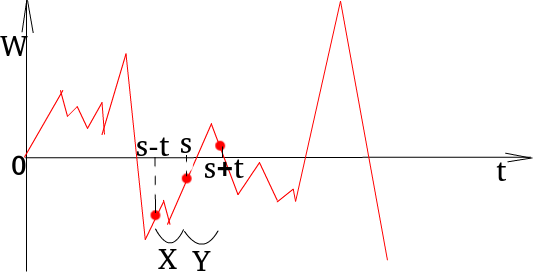
\includegraphics[width=.4\textwidth]{./pictures/5_6.png}
  \caption{График винеровского процесса}
  \label{fig:56}
\end{figure}

Есть 3 случайные величины.

У такого вектора есть плотность.
Случайные величины независимы
$$q_t =
  \iiint \limits_{x > y > z}
    p_{ \left( W \left( s \right), W \left( s - t \right), W \left( s + t \right) \right) }
      \left( x, y, z \right) dxdydz.$$

Вектор имеет нормальное распределение
$$ \begin{bmatrix}
    W \left( s \right) \\
    W \left( s - t \right) \\
    W \left( s + t \right)
  \end{bmatrix} \sim
  N \left(
    \left( \begin{bmatrix}
      0 \\
      0 \\
      0
    \end{bmatrix} \right),
    \left( \begin{bmatrix}
      s & s - t & s \\
      s - t & s - t & s - t \\
      s & s - t & s + t
    \end{bmatrix} \right) \right).$$

Нужно использовать какие-то свойства винеровского процесса.
Здесь нужно взять 2 приращения.
Эти приращения будут независимыми величинами с известным распределением $N \left( 0, t \right) $.

Вводим в рассмотрение приращения
$$ \begin{cases}
    X = W \left( s \right) - W \left( s - t \right), \\
    Y = W \left( s + t \right) - W \left( s \right).
  \end{cases}$$
Выразим из первого уравнения $W \left( s - t \right) = W \left( s \right) - X$,
а из второго --- $W \left( s + t \right) = W \left( s \right) + Y$.
Отнимем два последние уравнения
$$W \left( s + t \right) - W \left( s - t \right) =
  X + Y.$$
От всех частей неравенства в искомой вероятности вычтем $W \left( s - t \right) $
и заменим полученные выражения на введённые приращения
$$q_t =
  P \left\{
    W \left( s \right) - W \left( s - t \right) > 0 >
    W \left( s + t \right) - W \left( s - t \right) \right\} =
  P \left( X > 0 > X + Y \right).$$
Плотность вектора --- это произведение плотностей
$$P \left( X > 0 > X + Y \right) =
  \int \limits_{0}^{ \infty } \int \limits_{- \infty }^{-x}
    \frac{1}{2 \pi t} \cdot e^{-\frac{1}{2t} \left( x^2 + y^2 \right) } dydx =$$
Перейдём в полярную систему координат
$$x = r \cos \varphi, \,
  y = r \sin \varphi, \,
  dxdy = rdrd \varphi.$$
Получим
$$= \frac{1}{2 \pi t} \int \limits_0^{ \infty }
  \int \limits_{-\frac{ \pi }{2}}^{ \frac{ \pi }{4}} re^{-\frac{1}{2t} \cdot r^2} d \varphi dr =$$
Изобразим область интегрирования (рис. \ref{fig:561}).

\begin{figure}[h!]
  \centering
  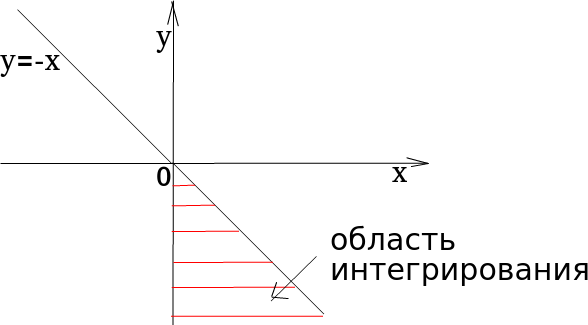
\includegraphics[width=.4\textwidth]{./pictures/5_6_1.png}
  \caption{Область интегрирования}
  \label{fig:561}
\end{figure}

По $ \varphi $ можем сразу проинтегрировать.
Интеграл по $ \varphi $ даст просто $ \frac{ \pi }{4}$.
Получаем
$$= \frac{1}{8} \int \limits_0^{ \infty } e^{-\frac{1}{2t} \cdot r^2} \cdot \frac{dr^2}{2t} =$$
Интеграл равен единице
$$= \frac{1}{8}$$

\addcontentsline{toc}{section}{Домашнее задание}
\section*{Домашнее задание}

\subsubsection*{5.12}

\textit{Задание.}
Пусть $ \left\{ W \left( t \right), \, t \geq 0 \right\} $ --- винеровский процесс.
Вычислите:
\begin{enumerate}[label=\alph*)]
  \item $M \left[
      \left( W \left( 4 \right) - 2W \left( 1 \right) + 2W \left( 2 \right) \right)^2 \right] $;
  \item $M \left[ \left( W \left( 1 \right) + 2W \left( 2 \right) + 1 \right)^3 \right] $;
  \item $M \left[ e^{W \left( 3 \right) - 2W \left( 2 \right) } \right] $;
  \item характеристическую функцию случайной величины $W \left( 1 \right) + 2W \left( 2 \right) + 1$.
\end{enumerate}

\textit{Решение.}
\begin{enumerate}[label=\alph*)]
  \item $W \left( 4 \right) - 2W \left( 1 \right) + W \left( 2 \right) =
    \xi \sim
    N \left( 0, 6 \right) $,
  потому что это линейная комбинация элементов гауссовского вектора.
  Найдём дисперссию
  $$D \xi =
    D \left[ W \left( 4 \right) - 2W \left( 1 \right) + W \left( 2 \right) \right] =
    cov \left( \xi, \xi \right) =$$
  Подставим выражения для случайной величины
  $$= cov \left[
      W \left( 4 \right) - 2W \left( 1 \right) + W \left( 2 \right),
      W \left( 4 \right) - 2W \left( 1 \right) + W \left( 2 \right) \right] =$$
  Воспользуемся линейностью
  \begin{gather*}
    = K \left( 4, 4 \right) - 2K \left( 4, 1 \right) + K \left( 4, 2 \right) -
    2K \left( 1, 4 \right) + 4K \left( 1, 1 \right) - 2K \left( 1, 2 \right) + \\
    + K \left( 2, 4 \right) - 2K \left( 2, 1 \right) + K \left( 2, 2 \right) = \\
    = 4 - 2 \cdot 1 + 2 - 2 \cdot 1 + 4 \cdot 1 - 2 \cdot 1 + 2 - 2 \cdot 1 + 2 =
    4 + 4 - 2 =
    6.
  \end{gather*}

  Нужно найти второй момент.
  $ \xi $ центрирована $M \xi^2 = D \xi = 6$;
  \item $W \left( 1 \right) + 2W \left( 2 \right) + 1 =
    \xi \sim
    N \left( 1, 5 \right) $,
  потому ято это линейная комбинация элементов гауссовского вектора.
  Найдём дисперсию.
  Константа на неё не влияет
  $D \xi =
    D \left[ W \left( 1 \right) - 2W \left( 2 \right) \right] =
    cov \left( \xi, \xi \right) $.
  Подставим выражения для случайной величины
  $$cov \left( \xi, \xi \right) =
    cov \left[
      W \left( 1 \right) + 2W \left( 2 \right) + 1,
      W \left( 1 \right) + 2W \left( 2 \right) + 1 \right] =$$
  Воспользуемся линейностью
  $$= \left( 1, 1 \right) + 2K \left( 1, 2 \right) + 2K \left( 2, 1 \right) +
    4K \left( 2, 2 \right) =
    1 + 2 + 2 + 8 =
    13.$$

  Нужно найти третий момент.
  $ \xi $ не центрирована.
  Нужно её центрировать $M \xi^3 = M \left[ \left( \xi - 1 \right) + 1 \right]^3$.
  Раскрываем скобки
  $$M \left[ \left( \xi - 1 \right) + 1 \right]^3 =
    M \left( \xi - 1 \right)^3 + 3M \left( \xi - 1 \right) + 3M \left( \xi - 1 \right) + 1 =$$
  По задаче 5.2 первое слагаемое --- 0, так как величина центрирована, второй момент --- 5,
  так как это дисперсия, первый момент --- ноль.
  Тогда
  $$= 0 + 3 \cdot 13 + 3 \cdot 0 + 1 = 38 + 1 = 40;$$
  \item $W \left( 3 \right) - 2W \left( 2 \right) = \xi \sim N \left( 0, 3 \right) $,
  потому что это линейная комбинация элементов гауссовского вектора.
  Найдём дисперсию
  $$D \xi =
    D \left[ W \left( 3 \right) - 2W \left( 2 \right) \right] =
    cov \left( \xi, \xi \right) =$$
  Подставим выражение для случайной величины
  $$= cov \left[
      W \left( 3 \right) - 2W \left( 2 \right), W \left( 3 \right) - 2W \left( 2 \right) \right] =$$
  Воспользуемся линейностью
  $$= K \left( 3, 3 \right) - 2K \left( 3, 2 \right) - 2K \left( 2, 3 \right) +
    4K \left( 2, 2 \right) =
    3 - 2 \cdot 2 - 2 \cdot 2 + 3 \cdot 2 =
    3.$$
  Нужно найти
  $$Me^{ \xi } =
    \int \limits_{ \mathbb{R}}
      \frac{1}{ \sqrt{6 \pi }} \cdot e^x \cdot p_{ \xi } \left( x \right) dx =
    \int \limits_{ \mathbb{R}}
      \frac{1}{6 \pi } \cdot e^x \cdot \frac{1}{6 \pi } \cdot e^{- \frac{x^2}{2 \cdot 9}} dx =
    \int \limits_{ \mathbb{R}} \frac{1}{ \sqrt{6 \pi }} \cdot e^{x - \frac{x^2}{18}} dx.$$
  Выделим полный квадрат в степени экспоненты
  $$ \frac{x^2}{18} - x =
    \frac{x^2}{ \left( 3 \sqrt{2} \right)^2} -
    2 \cdot \frac{1}{2} \cdot x \cdot \frac{1}{3 \sqrt{2}} \cdot 2 \sqrt{2} +
    \left( \frac{1}{2} \right)^2 \cdot \left( 2 \sqrt{2} \right)^2 =$$
  Три первых слагаемых образуют полный квадрат
  $$= \left( \frac{x}{3 \sqrt{2}} - \frac{3 \sqrt{2}}{2} \right)^2 + \frac{ 9 \cdot 2}{4} =
    \left( \frac{x}{3 \sqrt{2}} - \frac{3}{ \sqrt{2}} \right)^2 + \frac{9}{2} =
    \frac{ \left( x - 9 \right)^2}{2 \cdot 3} + \frac{9}{2}.$$
  Подставим полученное выражение в экспоненту
  $$ \int \limits_{ \mathbb{R}} \frac{1}{ \sqrt{6 \pi }} \cdot e^{x - \frac{x^2}{18}} dx =
    e^{- \frac{9}{2}}
    \int \limits_{ \mathbb{R}}
      \frac{1}{ \sqrt{6 \pi }} \cdot e^{- \frac{ \left( x - 9 \right)^2}{2 \cdot 9}} dx =$$
  Умножим и поделим на $ \sqrt{3}$ чтобы получить гауссовскую плотность
  $$= \sqrt{3} e^{- \frac{9}{2}}
    \int \limits_{ \mathbb{R}}
      \frac{1}{ \sqrt{2 \pi \cdot 9}} \cdot e^{-\frac{ \left( x - 9 \right)^2}{2 \cdot 9}} dx =$$
  Подинтергальная функция --- плотность нормального распределения,
  потому такой интеграл равен единице
  $$= \sqrt{3} e^{- \frac{9}{2}};$$
  \item нужно найти характеристическую функцию $W \left( 1 \right) + 2W \left( 2 \right) + 1$.

  Математическое ожидание такой величины равно 1, а дисперсия --- 13.
  Значит, получается
  $ \varphi_{W \left( 1 \right) =
    2W \left( 2 \right) + 1} \left( \lambda \right) =
    \varphi_{N \left( 1, 13 \right) } \left( \lambda \right) =
    e^{it - \frac{13t^2}{2}}$.
\end{enumerate}
